\chapter{ Констукторский раздел}
\label{cha:design}
    В данном разделе будут рассмотрены схемы алгоритмов, требования к функциональности ПО,
    и опредены способы тестирования.
    
    \section{Разработка алгоритмов}
        Ниже будут представлены схемы алгоритмов поиска растояния Левенштейна: \begin{enumerate}
            \item нерекурсивного с заполнением матрицы (рисунок \ref{schema:matr:Levenstein});
            \item рекурсивного без заполнения матрицы (рисунок \ref{schema:rec:Levenstein});
            \item рекурсивного с заполнением матрицы (рисунок \ref{schema:rec-matr:Levenstein}).
        \end{enumerate}

        Также будет представлена схема нерекурсивного алгоритма поиска растояния Дамерау-Левенштейна (рисунок \ref{schema:matr:Dameray-Levenstein}).

    \section{Требования к функциональности ПО}
        В данной работе требуется обеспечить следующую минимальную функциональность консольного приложения.
        \begin{enumerate}
            \item Режим ввода:
            \begin{enumerate}
                \item возможность считать две строки;
                \item вывод расстояний Левенштейна и Дамерау-Левенштейна между строками;
                \item вывод матриц, используемых в вычислении расстояний (если использовались).
            \end{enumerate}
            \item Экспериментальный режим: 
            \begin{enumerate}
                \item вывод таблицы с процессорным временем работы (Рисунок \ref{fig:1}).
            \end{enumerate}
        \end{enumerate}
        
        По умолчанию приложение работает в режиме ввода, для перехода в режим тестирования необходимо указать
        ключ -t при запуске. 

    \section{Тесты}
    Тестирование ПО будет проводиться методом чёрного ящика. Необходимо проверить работу системы 
    на тривиальных случаях (одна или обе строки пустые, строки полностью совпадают) 
    и несколько нетривальных случаев.

    \begin{figure}[h!]
        \centering
        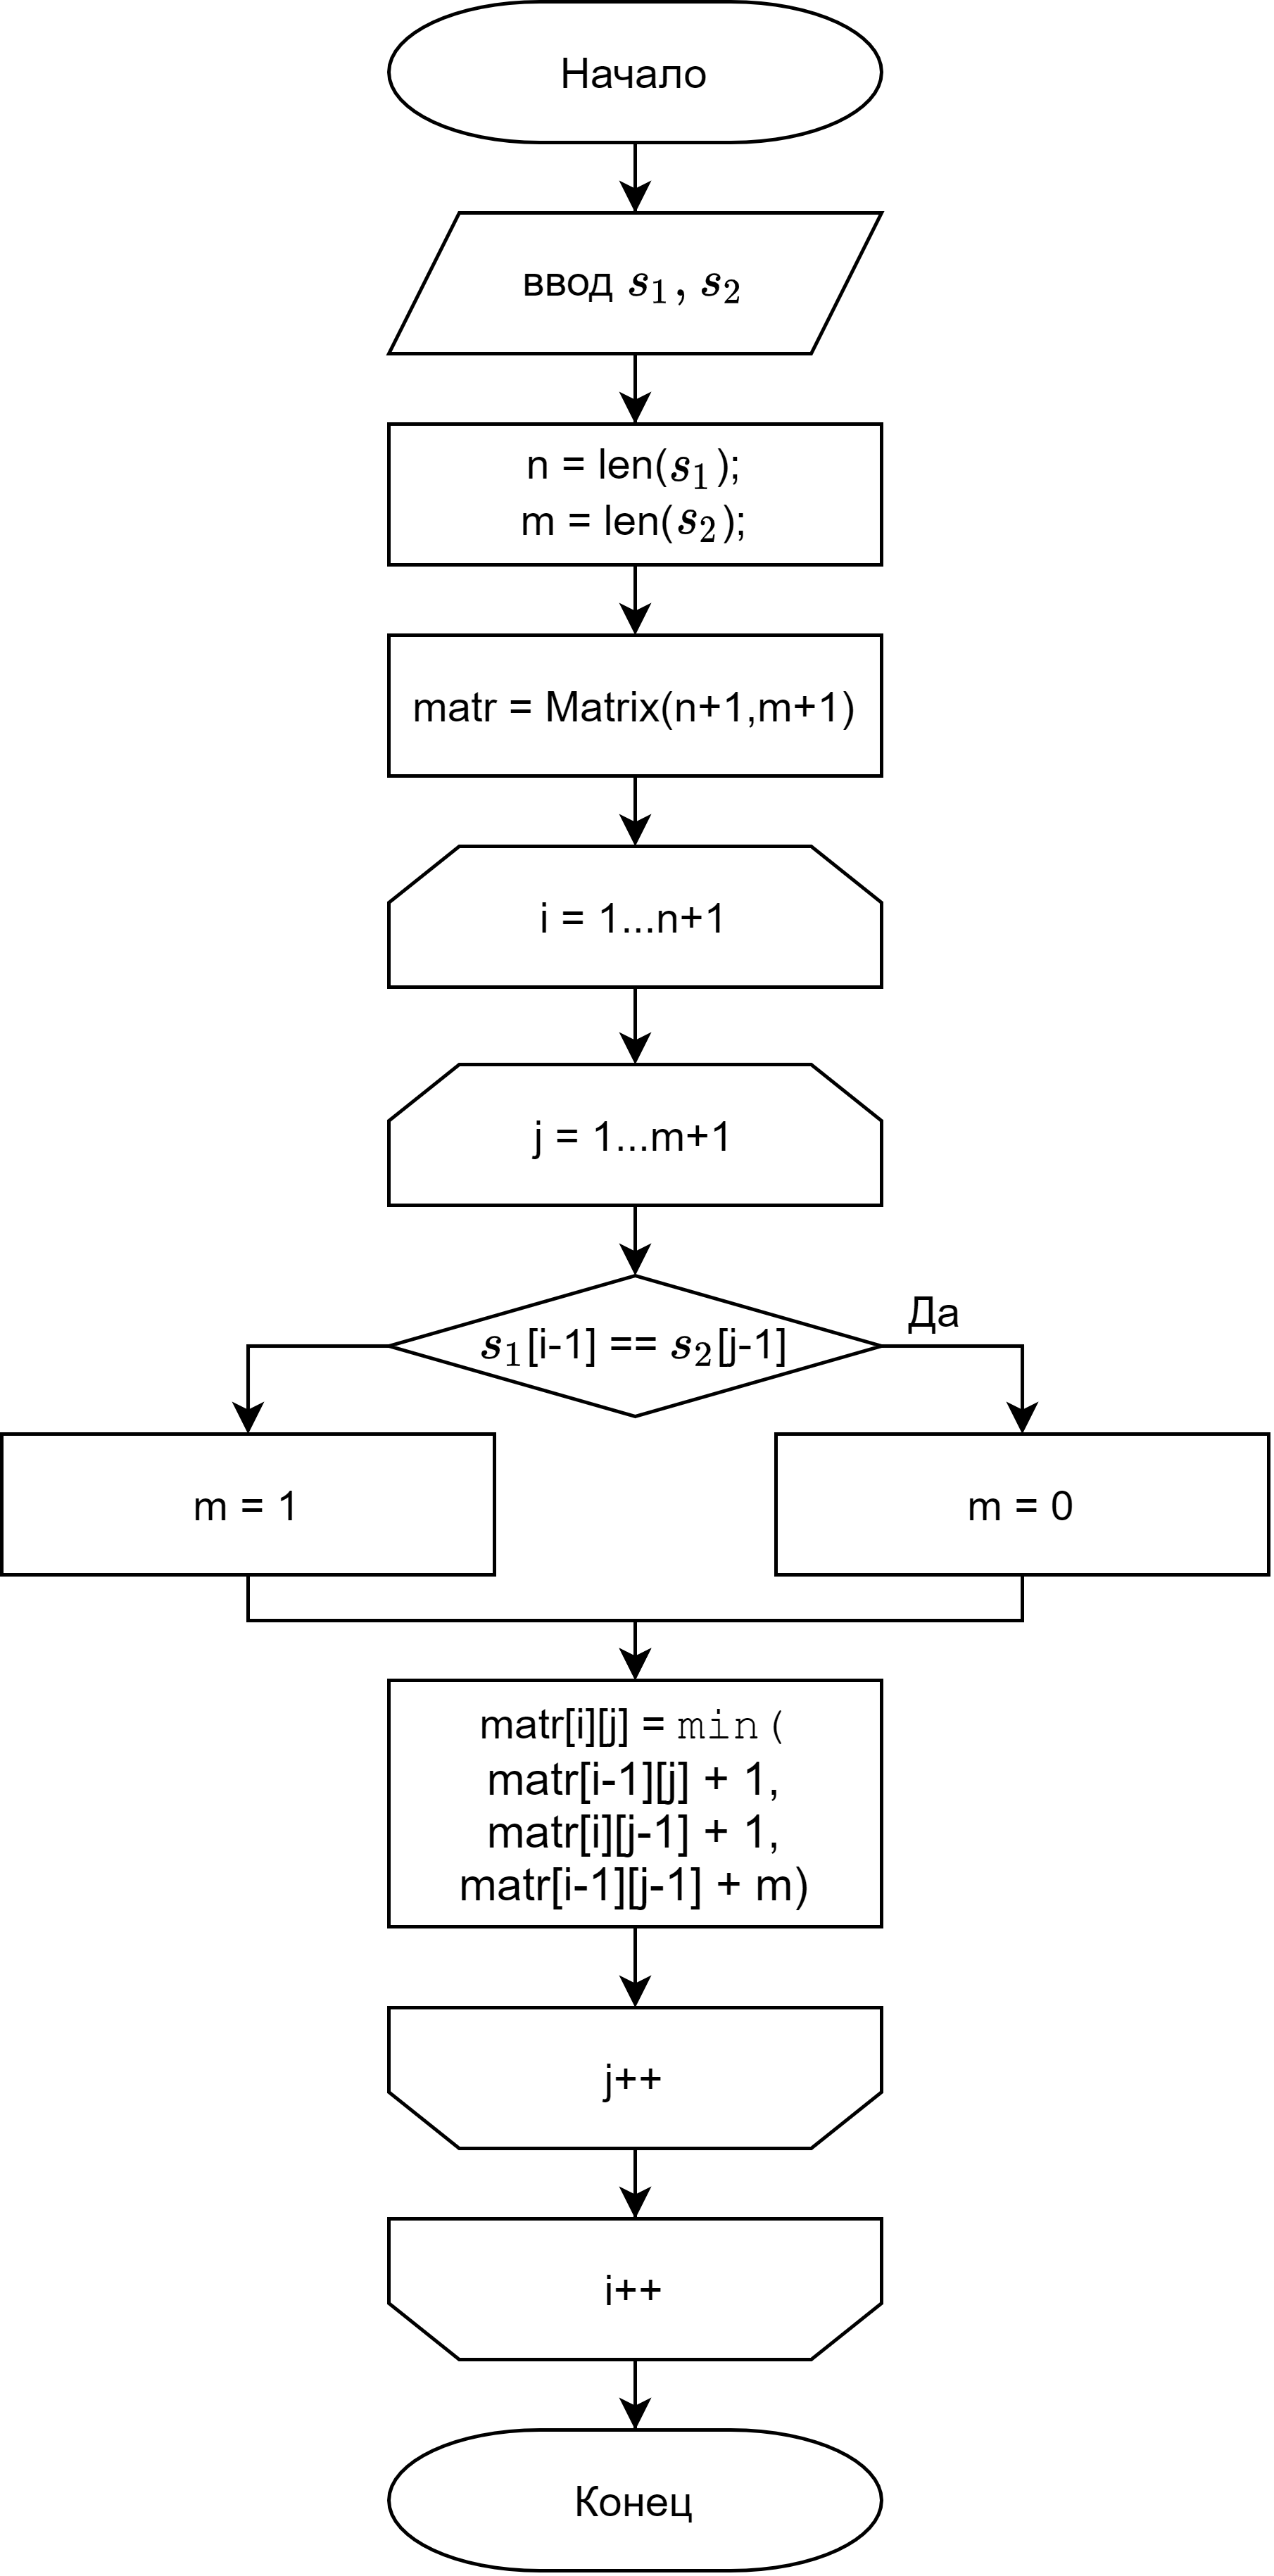
\includegraphics[scale=0.18]{LevMatr}
        \caption{Схема нерекурсивного поиска с заполнением матрицы}
        \label{schema:matr:Levenstein}
    \end{figure}

    \begin{figure}[h!]
        \centering
        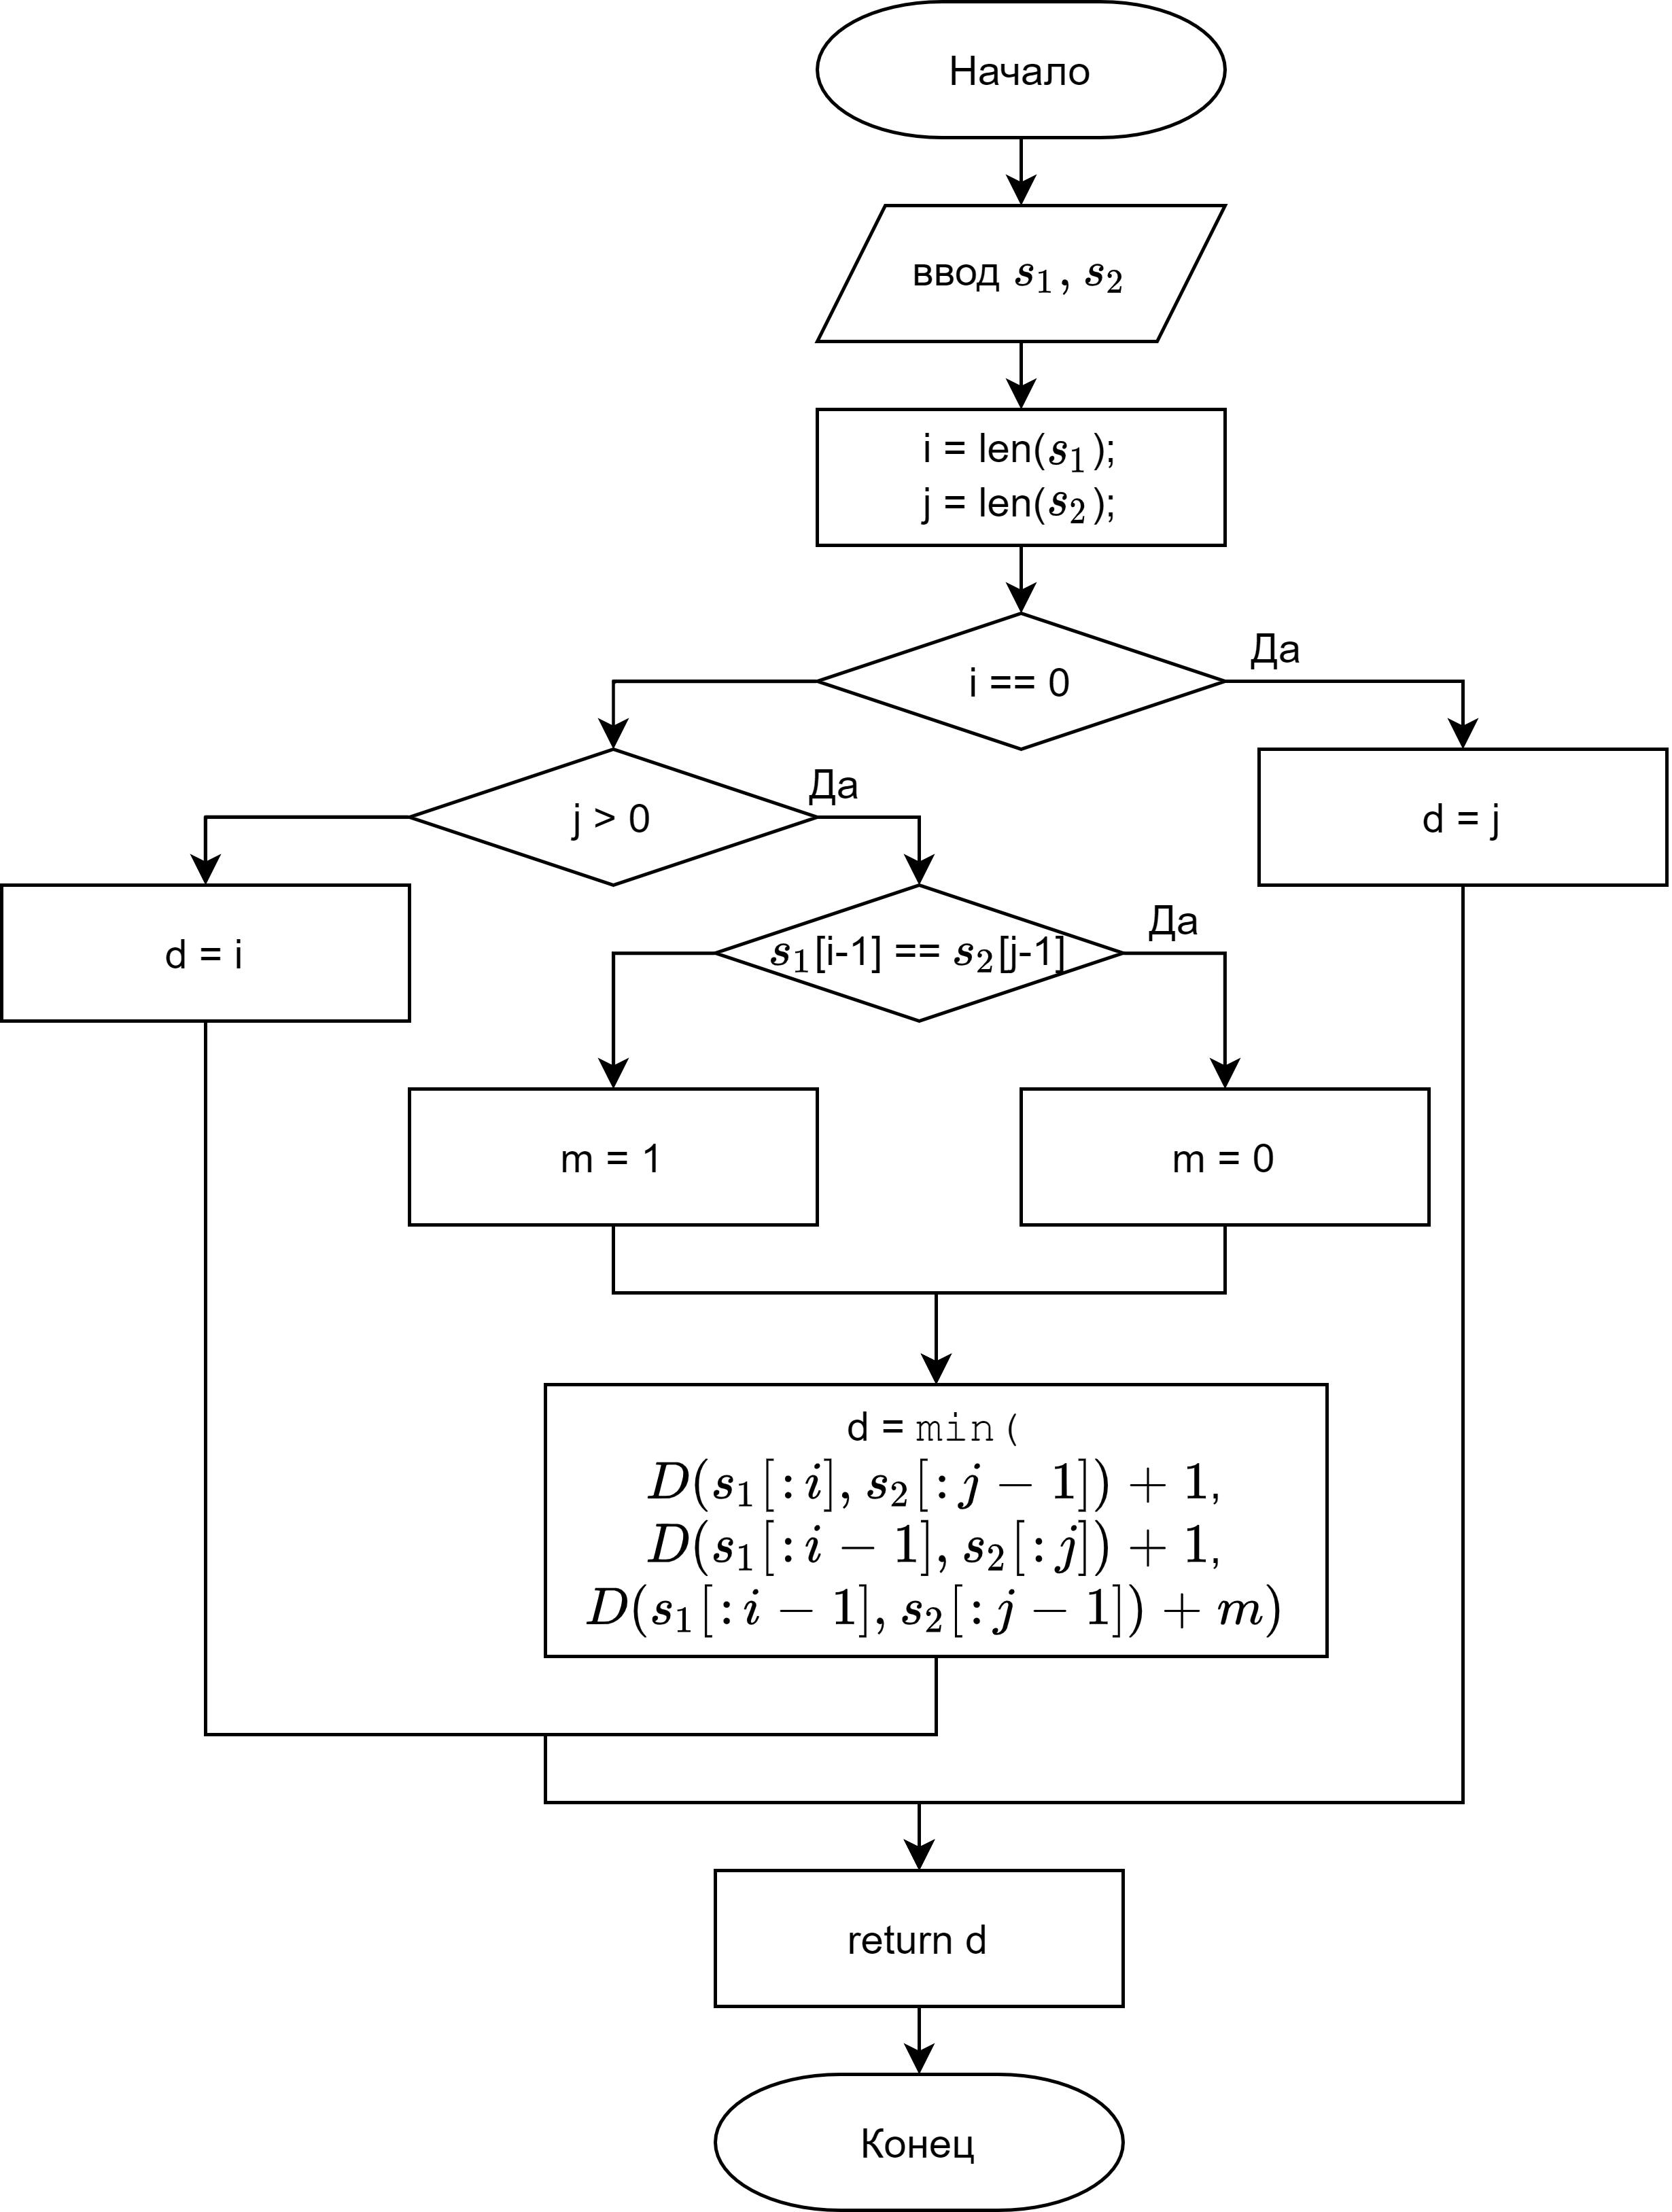
\includegraphics[scale=0.18]{LevRec}
        \caption{Схема рекурсивого поиска без заполнения матрицы}
        \label{schema:rec:Levenstein}
    \end{figure}

    \begin{figure}[h!]
        \centering
        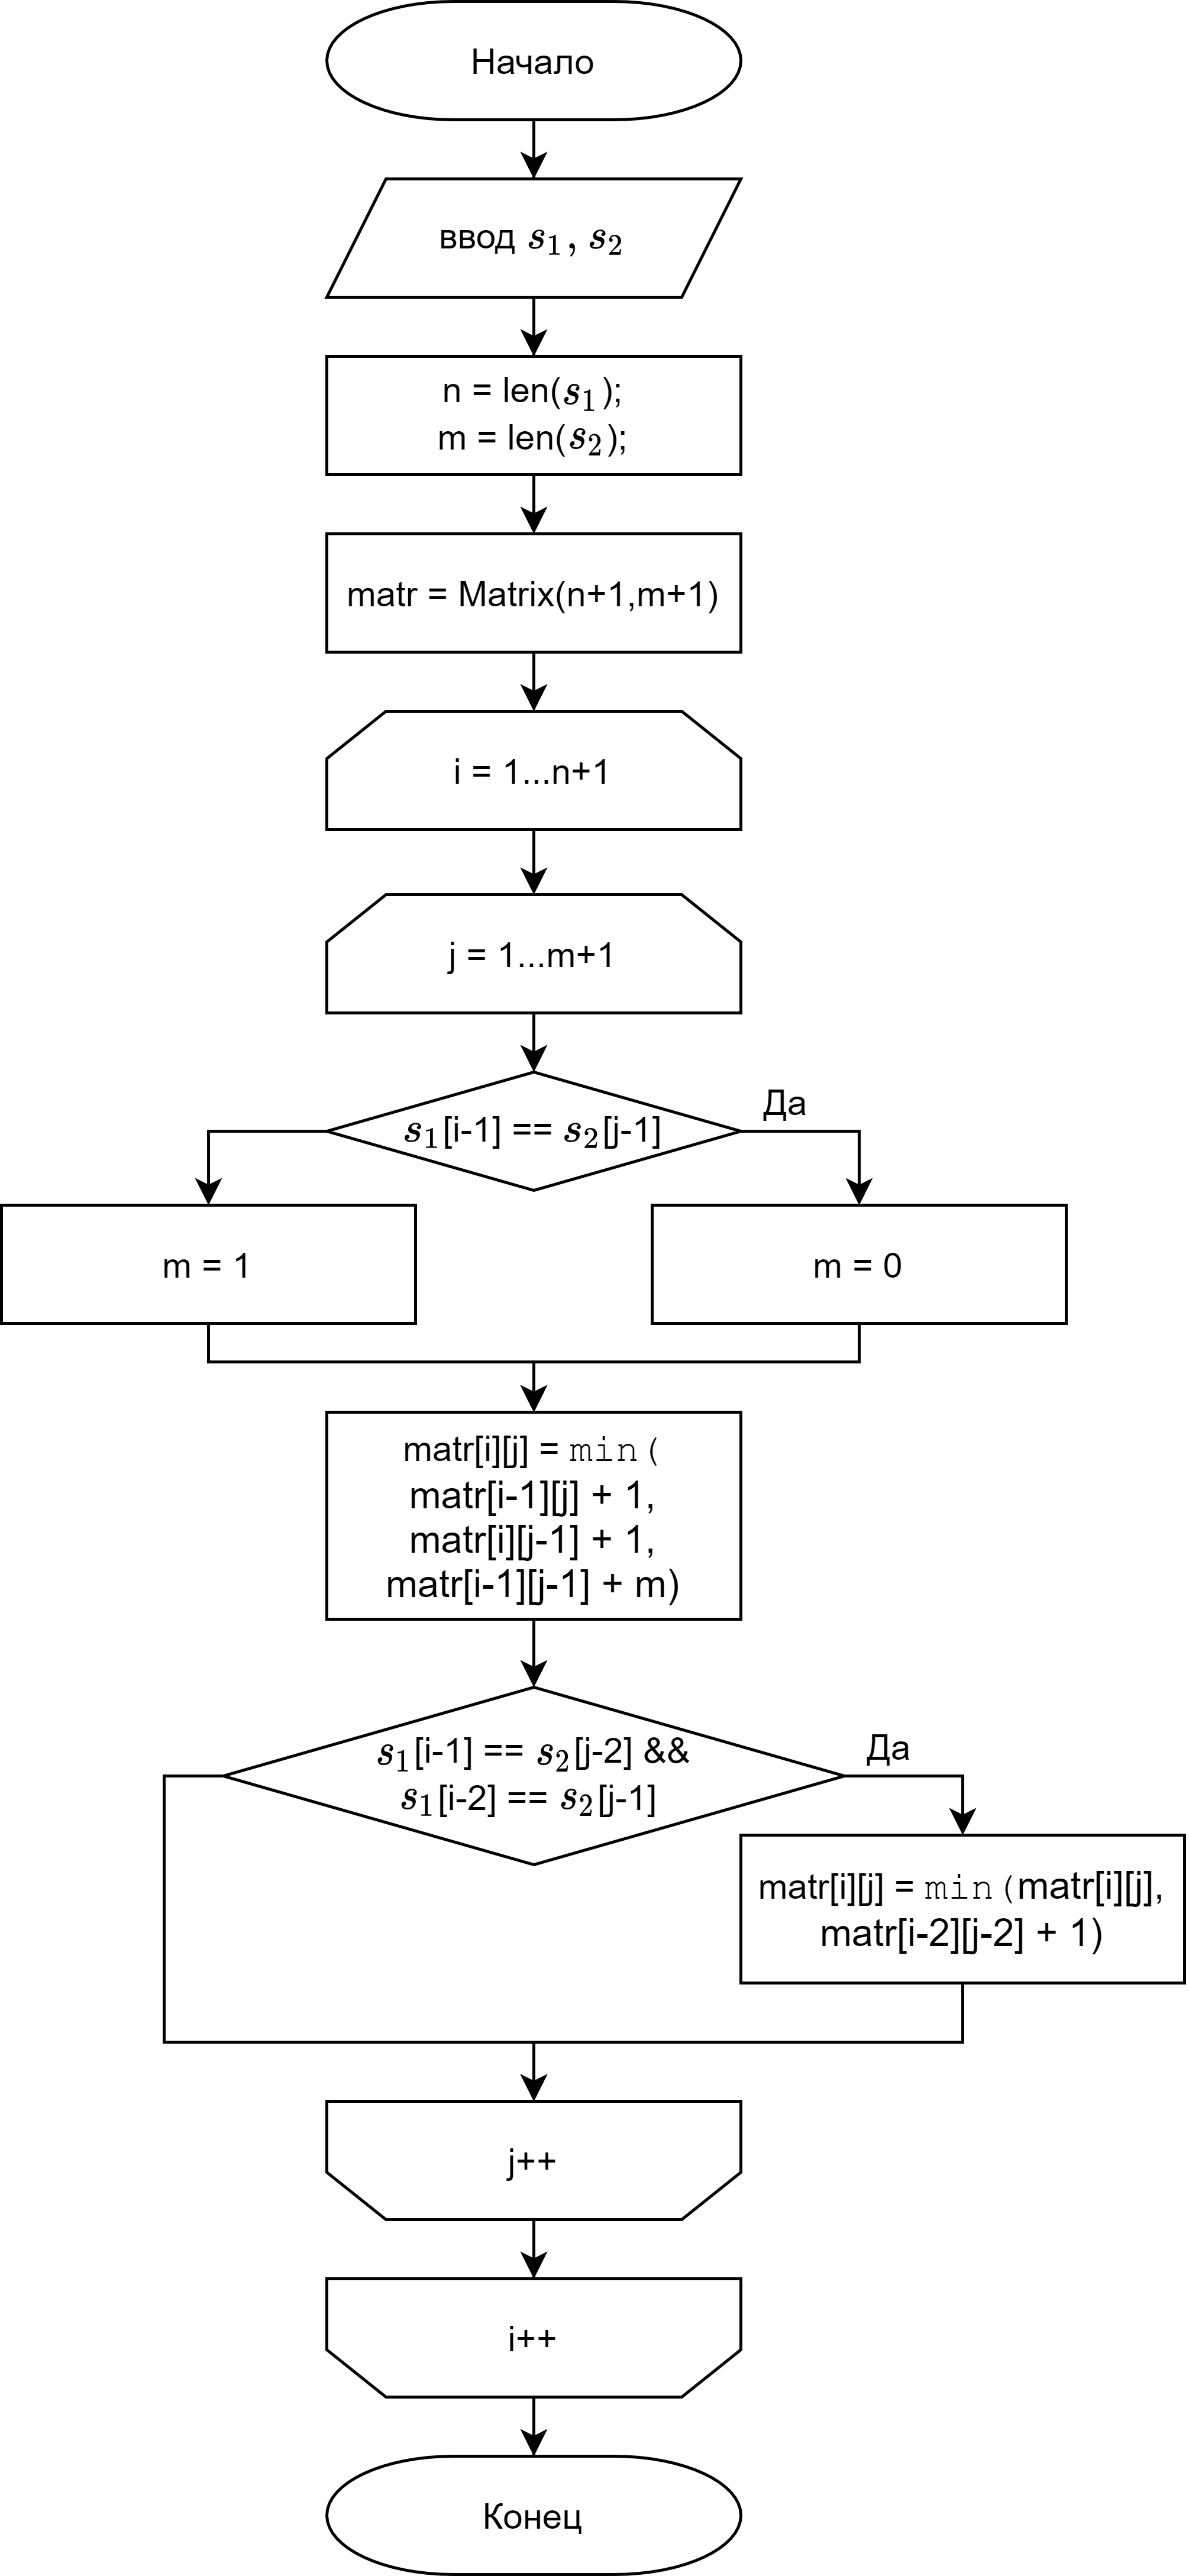
\includegraphics[scale=0.16]{DamLevMatr}
        \caption{Схема рекурсивого поиска с заполнением матрицы}
        \label{schema:rec-matr:Levenstein}
    \end{figure}

    \begin{figure}[h!]
        \centering
        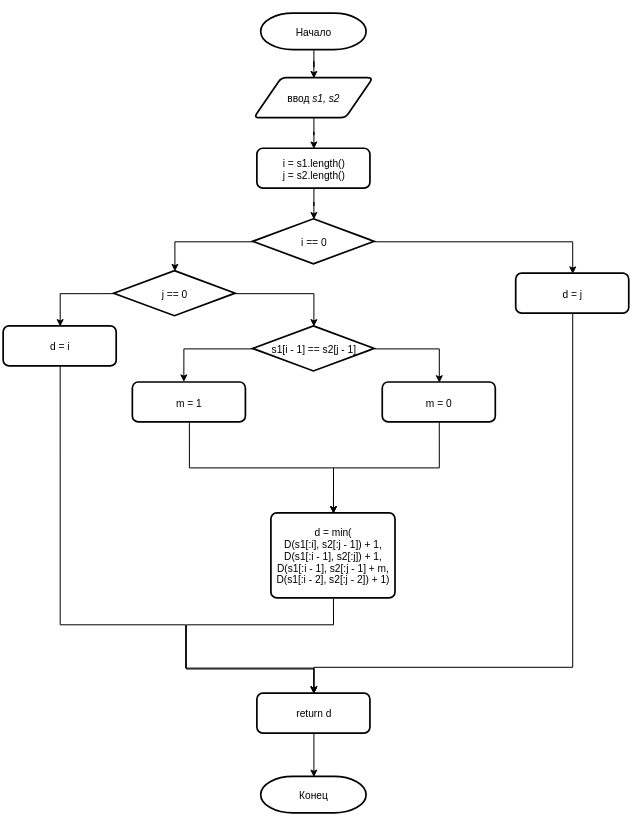
\includegraphics[scale=1]{LevGraph}
        \caption{Схема поиска р. Дамерау-Левенштейна}
        \label{schema:matr:Dameray-Levenstein}
    \end{figure}

\newpage